\chapter{KAJIAN PUSTAKA}

\section*{ }
Untuk mendukung penelitian ini, dibutuhkan beberapa teori penunjang sebagai bahan acuan dan referensi.
\vspace{1ex}

\section{Hasil Penelitian Terdahulu}
Penelitian mengenai identifikasi individu penyu laut telah berkembang dari pendekatan manual berbasis foto hingga sistem otomatis berbasis \textit{deep learning}.

\begin{enumerate}
\item \textbf{Pendekatan berbasis jaringan saraf awal.}
Carter et al.\ \cite{carter2014automated} merupakan salah satu peneliti pertama yang menerapkan jaringan saraf tiruan untuk keperluan identifikasi otomatis penyu laut. Mereka mengembangkan sistem Photo-ID berbasis citra sisik wajah (\textit{facial scute}) dengan memanfaatkan \textit{ensemble learning} jaringan saraf, dan mengujinya pada penyu hijau (\textit{Chelonia mydas}). Sistem tersebut menandai transisi paradigma dari pencocokan manual yang sangat bergantung pada keahlian pengamat menuju sistem otomatis yang lebih \textit{scalable} dan \textit{reproducible}.

\item \textbf{Validasi pola sisik sebagai penanda jangka panjang.}
Carpentier et al.\ \cite{carpentier2016stability} memvalidasi stabilitas pola sisik wajah pada penyu hijau selama rentang waktu hingga 11 tahun. Temuan tersebut memiliki signifikansi ilmiah yang tinggi karena mengonfirmasi bahwa sisik kepala dapat dimanfaatkan sebagai penanda identitas jangka panjang, sehingga memperkuat fondasi ilmiah bagi seluruh pendekatan Re-ID berbasis morfologi kepala penyu.
 
\item \textbf{Eksplorasi region identifikasi alternatif.}
Gatto et al.\ \cite{gatto2018flipper} mengusulkan pemanfaatan pola sisik pada sirip depan (\textit{front flipper}) sebagai alternatif maupun pelengkap terhadap sisik wajah, dengan menggunakan perangkat lunak APHIS (\textit{Automatic Photo Identification System}). Penelitian Dunbar et al.\ \cite{dunbar2023photo} selanjutnya membandingkan akurasi identifikasi menggunakan sisik kepala dengan sisik sirip, dan menyimpulkan bahwa sisik sirip memberikan akurasi yang lebih tinggi pada kondisi-kondisi tertentu, meskipun sisik kepala tetap menjadi pilihan utama dalam penelitian lapangan karena kemudahan pengambilan citra.
 
\item \textbf{Benchmark Re-ID berbasis \textit{deep learning}.}
Adam et al.\ \cite{adam2023seaturtleid2022} memperkenalkan dataset \textit{SeaTurtleID2022} yang memuat 8.729 foto dari 438 individu penyu loggerhead yang dikumpulkan selama 13 tahun di kepulauan Yunani. Dataset ini dilengkapi dengan protokol evaluasi \textit{time-aware open-set split} yang lebih representatif terhadap kondisi nyata dibandingkan pembagian acak konvensional. Mereka juga mengajukan sistem \textit{baseline} yang mengintegrasikan Hybrid Task Cascade untuk segmentasi kepala dengan ArcFace sebagai \textit{feature extractor}, sehingga mencapai akurasi Rank-1 sebesar 86{,}8\%.
 
\item \textbf{CNN untuk Re-ID penyu.}
Nguyen et al.\ \cite{nguyen2023cnn} mengevaluasi beberapa arsitektur CNN, meliputi AlexNet, GoogLeNet, VGG-19, dan ResNet-50, untuk keperluan identifikasi individu penyu berdasarkan citra sisik wajah. Dengan memanfaatkan 1.426 citra dari 20 kelas individu penyu, penelitian tersebut menunjukkan bahwa ResNet-50 mencapai akurasi 95{,}3\% pada dataset campuran, sementara AlexNet mencapai 97{,}74\% pada dataset berkualitas tinggi. Hasil ini membuktikan bahwa fitur sisik wajah memiliki tingkat diskriminasi yang memadai untuk CNN berbasis \textit{transfer learning}.
 
\item \textbf{\textit{Foundation model} untuk Re-ID satwa liar.}
\v{C}erm\'{a}k et al.\ \cite{cermak2024wildlifedatasets} memperkenalkan \textit{WildlifeDatasets}, yakni sebuah \textit{toolkit open-source} untuk Re-ID satwa liar beserta \textit{foundation model} pertama untuk Re-ID multi-spesies yang disebut MegaDescriptor. Model ini dilatih pada kumpulan dataset satwa liar berskala besar dan terbukti melampaui model pra-latih umum seperti CLIP dan DINOv2 secara signifikan pada berbagai dataset Re-ID satwa liar, termasuk dataset penyu. Perkembangan ini menandai pergeseran paradigma dari model \textit{species-specific} menuju model universal yang dapat digeneralisasi lintas spesies.
 
\item \textbf{Pemanfaatan kemiripan antar sisi wajah.}
Papafitsoros et al.\ \cite{papafitsoros2024facial} mengusulkan pendekatan baru yang memanfaatkan kemiripan visual antara profil kiri dan profil kanan dari individu yang sama, suatu aspek yang selama ini diabaikan dalam sistem Photo-ID konvensional. Dengan memanfaatkan metode berbasis fitur lokal dan \textit{deep embedding} (MegaDescriptor), pendekatan tersebut diuji pada empat dataset dari tiga spesies penyu yang berbeda, dan menunjukkan bahwa eksploitasi kemiripan antar sisi mampu meningkatkan akurasi Re-ID secara substansial.
\end{enumerate}

\section{Dasar Teori}
%-------------------------------------------------------------
\subsection{Re-Identifikasi}
%-------------------------------------------------------------
Re-identifikasi (\textit{re-identification}, Re-ID) merupakan tugas komputasi yang bertujuan untuk mengenali kembali suatu entitas, baik berupa individu, objek, maupun kendaraan, yang telah teramati sebelumnya berdasarkan ciri visual yang diekstraksi dari citra baru yang diambil dalam kondisi berbeda \cite{zheng2015scalable}. Berbeda dengan klasifikasi konvensional yang memetakan citra ke label kelas tetap, Re-ID beroperasi dalam skenario \textit{open-set}: model harus mampu membandingkan dua citra dan menentukan apakah keduanya berasal dari identitas yang sama, bahkan ketika identitas tersebut tidak pernah dijumpai selama proses pelatihan. Perbedaan mendasar inilah yang menjadikan Re-ID secara inheren lebih kompleks sekaligus lebih aplikatif dalam konteks dunia nyata dibandingkan dengan klasifikasi tertutup.
 
Secara prinsip, Re-ID dibangun di atas kerangka pembelajaran metrik (\textit{metric learning}). Model dilatih untuk memetakan setiap citra ke vektor \textit{embedding} dalam ruang berdimensi rendah sedemikian rupa sehingga dua citra dari entitas yang sama memiliki jarak yang kecil, sedangkan citra dari entitas yang berbeda memiliki jarak yang besar \cite{schroff2015facenet}. Prinsip tersebut dirumuskan sebagai:
\begin{equation}
    d\!\left(f(x_i),\, f(x_j)\right) \ll d\!\left(f(x_i),\, f(x_k)\right)
    \quad \forall\; y_i = y_j \neq y_k
\end{equation}
di mana $f(\cdot)$ adalah fungsi \textit{embedding} yang dipelajari, $d(\cdot,\cdot)$ adalah fungsi jarak (misalnya jarak Euclidean atau \textit{cosine distance}), dan $y$ adalah label identitas. Ruang \textit{embedding} yang berkualitas baik memiliki sifat bahwa operasi peringkatan (\textit{ranking}) berdasarkan jarak berbanding lurus dengan kemiripan identitas, sehingga pencarian tetangga terdekat menghasilkan identitas yang tepat.
 
Mekanisme kerja sistem Re-ID secara umum melibatkan dua tahap utama, yaitu: (1) tahap \textit{embedding}, di mana setiap citra \textit{query} maupun \textit{gallery} diproses oleh model untuk menghasilkan vektor representasi; dan (2) tahap \textit{retrieval}, di mana kemiripan antara vektor \textit{query} dan seluruh vektor \textit{gallery} dihitung, kemudian kandidat identitas diurutkan berdasarkan kemiripan tersebut \cite{zhong2017reranking}. Identitas yang paling sering muncul pada posisi teratas ditetapkan sebagai prediksi identitas \textit{query}. Evaluasi sistem dilakukan menggunakan metrik \textit{Cumulative Matching Characteristic} (CMC) dan \textit{Mean Average Precision} (mAP), yang secara berturut-turut mengukur ketepatan peringkat teratas dan kualitas keseluruhan urutan hasil pencarian \cite{zheng2015scalable}.
 
% Pendekatan Re-ID berbasis \textit{metric learning} dipilih dalam penelitian ini karena dataset penyu yang tersedia memiliki keterbatasan jumlah citra per individu dan terdapat individu-individu baru yang tidak dijumpai selama pelatihan. Paradigma klasifikasi tertutup tidak dapat mengakomodasi individu baru tanpa melatih ulang seluruh model, sedangkan Re-ID berbasis \textit{metric learning} memungkinkan identifikasi individu baru cukup dengan menambahkan vektor \textit{embedding}-nya ke dalam galeri tanpa perubahan parameter model apapun.
 
Re-ID telah diterapkan secara luas di berbagai domain. Dalam keamanan publik dan pengawasan (\textit{surveillance}), Re-ID digunakan untuk melacak individu melintasi jaringan kamera yang tidak tumpang tindih (\textit{non-overlapping cameras}) \cite{zheng2015scalable}. Dalam ranah transportasi, Re-ID kendaraan dimanfaatkan untuk memantau pergerakan kendaraan di jaringan jalan raya, mendukung aplikasi seperti deteksi kendaraan curian dan analisis arus lalu lintas jangka panjang. Di bidang medis, Re-ID diterapkan untuk mencocokkan data pasien lintas sesi pencitraan. Di bidang olahraga, Re-ID atlet digunakan untuk analisis taktik pertandingan dan pelacakan pergerakan pemain dari berbagai sudut kamera.
 
Aplikasi yang semakin berkembang pesat adalah Re-ID untuk pemantauan satwa liar, di mana sistem digunakan untuk mengidentifikasi individu hewan dari foto lapangan tanpa memerlukan penanda fisik yang invasif \cite{cermak2024wildlifedatasets}. Contoh aplikasi mencakup identifikasi paus bungkuk dari pola unik sirip ekornya, identifikasi hiu paus dari pola bintik, identifikasi harimau dari garis-garis kulit, hingga identifikasi penyu laut dari pola sisik kepala \cite{adam2023seaturtleid2022}.

\subsubsection{Re-identifikasi Individu Satwa}
 
Re-identifikasi individu satwa liar (\textit{individual wildlife re-identification}) merupakan penerapan khusus Re-ID dalam rangka pemantauan populasi hewan secara non-invasif \cite{schneider2020deep}. Alih-alih memasang penanda fisik seperti \textit{pit-tag}, gelang, atau pemancar yang berpotensi menimbulkan stres, luka, maupun perubahan perilaku pada hewan, sistem Re-ID berbasis kamera memanfaatkan ciri visual alami seperti pola bulu, tekstur kulit, atau bentuk tubuh untuk membedakan dan melacak individu \cite{clapham2021perspectives}. Metode ini bersifat non-invasif secara fundamental karena hanya memerlukan foto biasa yang dapat diambil dari jarak aman.
 
Dari perspektif ekologis, kemampuan melacak individu secara akurat dan berkesinambungan sangat esensial untuk mengestimasi ukuran populasi melalui metode \textit{capture-mark-recapture} (CMR), memahami pola migrasi musiman, menganalisis perilaku sosial dan reproduksi, serta merancang strategi konservasi berbasis bukti yang dapat dipertanggungjawabkan \cite{clapham2021perspectives}. Dibandingkan dengan penandaan fisik, sistem Re-ID otomatis juga memiliki keunggulan dalam kapabilitas retrospektif: foto-foto lama yang tersimpan dalam arsip dapat dicocokkan dengan individu-individu yang baru diidentifikasi, sehingga data historis yang sebelumnya tidak termanfaatkan dapat dioptimalkan kembali.
 
% Tantangan utama dalam Re-ID satwa liar dibandingkan dengan Re-ID manusia mencakup: (1) variasi pose yang ekstrem akibat pergerakan hewan yang bebas dan tidak terkontrol; (2) kondisi pencahayaan dan latar belakang yang sangat bervariasi bergantung pada habitat dan waktu pengambilan foto; (3) keterbatasan data mengingat setiap individu hewan mungkin hanya terekam dalam sejumlah kecil foto sepanjang program pemantauan; serta (4) kebutuhan generalisasi terhadap spesies, populasi, atau lokasi geografis baru yang tidak tercakup dalam dataset pelatihan \cite{cermak2024wildlifedatasets}. Tantangan terakhir yang dikenal sebagai \textit{cross-domain generalization} menjadi fokus khusus dalam penelitian ini, di mana model yang dilatih pada satu populasi penyu harus mampu diuji pada populasi yang berbeda secara geografis.

%-------------------------------------------------------------
\subsection{Ekstraksi Pola Kepala Penyu}
%-------------------------------------------------------------
\subsubsection{Karakteristik Pola Sisik Kepala Penyu}
 
Kepala penyu laut ditutupi oleh sisik-sisik yang disebut \textit{scutes}, yang tersusun dalam pola geometris yang kompleks dan unik pada setiap individu \cite{carpentier2016stability}. Pola tersebut terbentuk selama masa embrio dan tidak mengalami perubahan yang signifikan sepanjang hayat hewan, sehingga berfungsi sebagai penanda biometrik alami yang persisten \cite{carter2014automated}. Setiap sisik memiliki bentuk, ukuran, dan posisi relatif yang khas; kombinasi seluruh sisik pada satu sisi kepala menghasilkan sidik jari yang unik per individu.
 
Kedua sisi kepala penyu, yakni profil kiri dan profil kanan, memiliki pola sisik yang berbeda satu sama lain bahkan pada individu yang sama \cite{papafitsoros2024facial}. Kondisi ini mengharuskan sistem Photo-ID tradisional untuk memisahkan perpustakaan citra berdasarkan sisi, yang pada gilirannya mengurangi jumlah data yang tersedia untuk pencocokan. Penelitian terkini menunjukkan bahwa meskipun berbeda, kedua profil tersebut memiliki kemiripan visual yang dapat dieksploitasi untuk meningkatkan akurasi identifikasi \cite{papafitsoros2024facial}.

\begin{figure}[H]
	\centering
	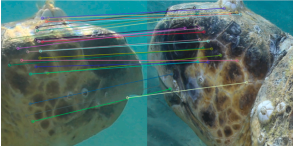
\includegraphics[width=0.5\linewidth]{bab2/face-scale.png}
	\caption{Persamaan pola di sisik kepala pada individu penyu yang sama \cite{papafitsoros2024facial}}
	\label{fig:face-scale}
\end{figure}

\subsubsection{Metode Ekstraksi Fitur Berbasis Citra Kepala}
 
Secara historis, ekstraksi fitur dari citra kepala penyu dilakukan menggunakan deskriptor fitur lokal seperti SIFT (\textit{Scale-Invariant Feature Transform}), SURF (\textit{Speeded-Up Robust Features}), atau ORB (\textit{Oriented FAST and Rotated BRIEF}) yang mendeteksi dan mendeskripsikan titik-titik kunci (\textit{keypoints}) pada tepi dan persimpangan sisik \cite{adam2023seaturtleid2022}. Metode-metode tersebut kemudian diimplementasikan dalam perangkat lunak khusus seperti APHIS \cite{gatto2018flipper} dan HotSpotter \cite{dunbar2023photo}.
 
Pendekatan berbasis \textit{deep learning} menggantikan ekstraksi fitur manual dengan representasi yang dipelajari secara otomatis dari data. CNN yang dilatih dengan \textit{transfer learning} dari ImageNet \cite{nguyen2023cnn} mampu mengekstraksi fitur hierarkis yang lebih kaya: lapisan-lapisan awal menangkap tepi dan tekstur sisik, sementara lapisan-lapisan dalam mengodekan pola geometris kompleks yang khas per individu. Pada arsitektur ViT \cite{dosovitskiy2021image}, mekanisme \textit{self-attention} memungkinkan model untuk secara serentak memperhatikan beberapa region sisik yang tersebar di seluruh kepala, sehingga menghasilkan representasi global yang lebih komprehensif dibandingkan CNN.

%-------------------------------------------------------------
\subsection{Vision Transformer}
%-------------------------------------------------------------
\textit{Vision Transformer} (ViT) merupakan arsitektur jaringan saraf yang diadaptasi dari arsitektur \textit{Transformer} yang semula dikembangkan untuk pemrosesan bahasa alami, kemudian diterapkan secara langsung pada data citra \cite{dosovitskiy2021image}. Dosovitskiy et al.\ menunjukkan bahwa sebuah \textit{Transformer} murni yang diterapkan pada urutan \textit{patch} citra mampu mencapai akurasi yang setara atau bahkan melampaui jaringan konvolusi (\textit{convolutional neural networks}, CNN) terbaik pada tugas klasifikasi citra, dengan catatan bahwa model dilatih pada data yang memadai dalam jumlah besar. Perbedaan mendasar ViT dengan CNN terletak pada tidak adanya \textit{inductive bias} spasial seperti lokalitas dan translasi-invariansi yang dimiliki konvolusi, sehingga ViT harus mempelajari hubungan spasial secara murni dari data.

\begin{figure}[H]
	\centering
	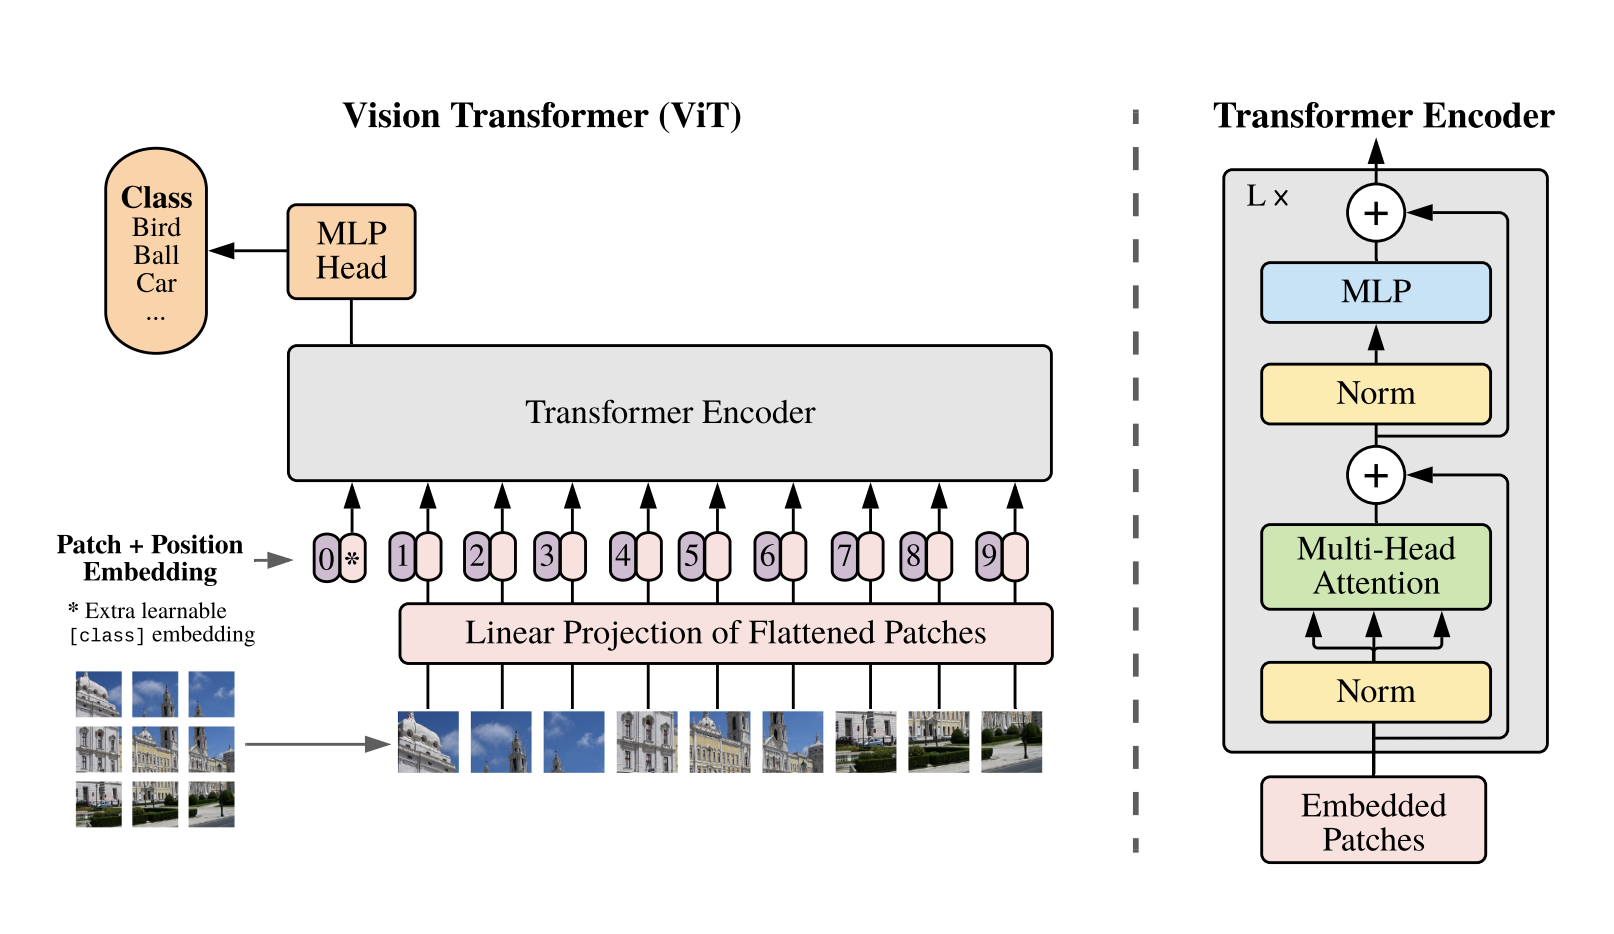
\includegraphics[width=0.9\linewidth]{bab2/vit-architecture.png}
	\caption{Arsitektur ViT: pembagian citra menjadi \textit{patch} sebelum diproses oleh lapisan \textit{transformer}. \cite{dosovitskiy2021image}}
	\label{fig:vit-architecture}
\end{figure}

%-------------------------------------------------------------
\subsection{Mekanisme Pembagian Patch}
%-------------------------------------------------------------
Citra masukan berukuran $H \times W \times C$ dibagi menjadi $N = \frac{H \cdot W}{P^2}$ \textit{patch} berukuran $P \times P$ piksel, di mana $P$ adalah ukuran \textit{patch}. Setiap \textit{patch} diratakan (\textit{flatten}) menjadi vektor berdimensi $P^2 \cdot C$, kemudian diproyeksikan secara linear ke dimensi laten $D$ menggunakan matriks proyeksi yang dapat dipelajari, sehingga menghasilkan urutan $N$ vektor \textit{embedding patch} \cite{dosovitskiy2021image}. Informasi posisi spasial setiap \textit{patch} ditambahkan melalui \textit{positional embedding} yang dapat dipelajari, agar model mengetahui lokasi relatif setiap \textit{patch} dalam citra asli.
 
Sebuah token kelas (\textit{class token}, \texttt{[CLS]}) yang dapat dipelajari ditambahkan di awal urutan, menghasilkan urutan total sepanjang $N+1$ token. Token ini tidak berkorespondensi dengan \textit{patch} citra mana pun, melainkan berinteraksi dengan seluruh \textit{patch} melalui \textit{self-attention} dan mengakumulasikan informasi global dari keseluruhan citra \cite{dosovitskiy2021image}. Setelah melewati seluruh blok \textit{Transformer}, keluaran dari token \texttt{[CLS]} inilah yang dimanfaatkan sebagai representasi global citra untuk tugas hilir, termasuk Re-ID. %Dalam penelitian ini, ukuran \textit{patch} $P = 16$ digunakan, sehingga untuk citra $256 \times 256$, model memproses urutan 257 token (256 \textit{patch} + 1 \texttt{[CLS]}).

\subsubsection{Blok Transformer dan Self-Attention}
 Setiap blok \textit{Transformer} dalam ViT terdiri dari dua sub-lapisan utama yang diapit oleh \textit{Layer Normalization} (LN) dan koneksi residual, yaitu: (1) \textit{Multi-Head Self-Attention} (MHSA) dan (2) \textit{Multi-Layer Perceptron} (MLP) dengan aktivasi GELU. Mekanisme \textit{self-attention} memungkinkan setiap token untuk mempertimbangkan kontribusi semua token lain dalam urutan secara global dan simultan, tanpa batasan jangkauan (\textit{receptive field}) seperti yang terdapat pada operasi konvolusi \cite{dosovitskiy2021image}.

Pada MHSA dengan $h$ \textit{head}, setiap token diproyeksikan menjadi tiga vektor Query ($Q$), Key ($K$), dan Value ($V$). Skor \textit{attention} antara setiap pasang token dihitung sebagai:
\begin{equation}
    \text{Attention}(Q, K, V)
    = \text{softmax}\!\left(\frac{QK^\top}{\sqrt{d_k}}\right) V
\end{equation}
di mana $d_k$ adalah dimensi tiap \textit{head}. Pemanfaatan beberapa \textit{head} secara paralel memungkinkan model untuk mempelajari pola relasi yang beragam secara simultan; misalnya, satu \textit{head} dapat belajar memperhatikan tepi sisik sementara \textit{head} lain memperhatikan pola warna. Kemampuan MHSA untuk memandang keseluruhan citra secara global pada setiap lapisan sangat relevan untuk Re-ID penyu, di mana pola diskriminatif tersebar di berbagai region sisik kepala yang tidak berdekatan.

%-------------------------------------------------------------
\subsection{Pra-pelatihan DINO}
%-------------------------------------------------------------
DINO (\textit{Self-DIstillation with NO labels}) adalah kerangka pra-pelatihan \textit{self-supervised} yang dirancang khusus untuk bersinergi dengan arsitektur \textit{Vision Transformer} \cite{caron2021dino}. \textit{Self-supervised learning} (SSL) adalah paradigma pelatihan di mana model belajar merepresentasikan data tanpa memerlukan anotasi label dari manusia, melainkan dengan memanfaatkan struktur inheren dari data itu sendiri sebagai sinyal supervisi. Keuntungan fundamental SSL adalah kemampuannya memanfaatkan dataset citra yang jauh lebih besar dibandingkan dataset berlabel, yang secara umum menghasilkan representasi yang lebih kaya dan lebih dapat digeneralisasi lintas domain. Keluarga DINO telah berkembang dari versi aslinya (DINO, 2021) hingga DINOv2 (2023) yang jauh lebih kuat, keduanya dikembangkan oleh Facebook AI Research (FAIR).
 
\subsubsection{DINO}
 
DINO diusulkan oleh Caron et al.\ \cite{caron2021dino} dengan tujuan untuk memahami apakah pelatihan \textit{self-supervised} dapat membangkitkan properti-properti unik yang tidak muncul ketika ViT dilatih secara \textit{supervised}. DINO menggunakan kerangka \textit{teacher-student self-distillation}: dua jaringan dengan arsitektur identik, yakni \textit{student} dan \textit{teacher}, secara bersamaan menerima \textit{crop} berbeda dari citra yang sama, dan model \textit{student} dilatih untuk mencocokkan distribusi keluaran \textit{softmax} dari model \textit{teacher}. Model \textit{teacher} tidak dilatih secara langsung, melainkan diperbarui sebagai \textit{exponential moving average} (EMA) dari bobot \textit{student}, sehingga tidak memerlukan label eksternal maupun \textit{negative pair} seperti yang digunakan dalam metode kontrastif.
 
Fungsi \textit{loss} DINO meminimalkan \textit{cross-entropy} antara distribusi keluaran \textit{student} dan \textit{teacher} pada pasangan \textit{global} dan \textit{local crop}:
\begin{equation}
    \mathcal{L}_{\text{DINO}}
    = -\sum_{x \in \{\text{global crops}\}}
      \sum_{\substack{x' \in \{\text{all crops}\} \\ x' \neq x}}
      P_s(x')\, \log P_t(x)
\end{equation}
di mana $P_s$ dan $P_t$ adalah distribusi \textit{softmax} yang dinormalisasi dari \textit{student} dan \textit{teacher} dengan parameter temperatur yang berbeda \cite{caron2021dino}.
 
Caron et al.\ \cite{caron2021dino} mengidentifikasi dua sifat \textit{emerging} yang penting: pertama, modul \textit{self-attention} pada blok terakhir secara eksplisit mengandung informasi mengenai tata letak skenario dan batas objek semantik, bahkan pada resolusi piksel, tanpa pernah diberikan label segmentasi; kedua, fitur yang dihasilkan merupakan \textit{k-NN classifier} yang sangat baik, mencapai 78{,}3\% akurasi top-1 pada ImageNet tanpa pelatihan lapisan klasifikasi apapun. Properti pertama sangat relevan untuk Re-ID penyu, karena kemampuan membedakan batas antar sisik kepala tanpa anotasi manual merupakan keunggulan yang signifikan mengingat tidak tersedianya dataset penyu berlabel segmentasi sisik secara individual.

\subsubsection{DINOv2}
 
DINOv2 diusulkan oleh Oquab et al.\ \cite{oquab2023dinov2} sebagai evolusi signifikan dari DINO yang menjawab dua kelemahan utamanya: keterbatasan skala data pelatihan dan inkonsistensi kualitas representasi antar tugas. Perbedaan utamanya terletak pada tiga aspek: (1) \textit{pipeline} kurasi data otomatis berbasis \textit{retrieval} yang membangun dataset LVD-142M, yakni 142 juta citra berkualitas tinggi dan beragam dari sumber web tanpa label; (2) teknik pelatihan gabungan yang mengombinasikan fungsi \textit{loss} DINO dengan komponen iBOT (\textit{image-level} dan \textit{patch-level self-distillation}) untuk menghasilkan fitur global dan lokal yang sama-sama kuat; serta (3) berbagai teknik stabilisasi pelatihan yang memungkinkan pelatihan pada skala besar tanpa divergensi \cite{oquab2023dinov2}.
 
Oquab et al.\ \cite{oquab2023dinov2} menunjukkan bahwa DINOv2 menghasilkan fitur visual serba guna (\textit{all-purpose visual features}) yang dapat digunakan secara langsung tanpa \textit{fine-tuning} untuk berbagai tugas, meliputi klasifikasi, deteksi objek, segmentasi semantik, hingga estimasi kedalaman monokuler. Pada hampir seluruh \textit{benchmark} yang diuji, DINOv2 melampaui metode \textit{self-supervised} sebelumnya dan bersaing dengan atau bahkan melampaui model yang dilatih secara \textit{weakly supervised} menggunakan data berskala web berlabel teks.
 
\subsubsection{DINOv3}
 
DINOv3 diperkenalkan oleh Sim\'{e}oni et al.\ \cite{simeoni2025dinov3} sebagai generasi lanjutan dari keluarga DINO yang berfokus pada peningkatan kualitas representasi visual universal untuk berbagai tugas \textit{computer vision}. Berbeda dengan DINOv2 yang menitikberatkan pada pembangunan fitur visual serbaguna melalui kombinasi \textit{image-level} dan \textit{patch-level self-distillation}, DINOv3 dikembangkan untuk menghasilkan representasi yang lebih stabil, lebih kaya secara semantik, dan lebih kuat dalam memahami struktur spasial lokal pada citra.
 
Seperti pendahulunya, DINOv3 tetap menggunakan paradigma \textit{teacher-student self-distillation} berbasis Vision Transformer (ViT), di mana model \textit{teacher} diperbarui menggunakan mekanisme EMA dari parameter \textit{student} \cite{simeoni2025dinov3}. Namun demikian, DINOv3 memperkenalkan berbagai penyempurnaan pada strategi pelatihan dan regularisasi sehingga mampu menghasilkan fitur yang lebih konsisten pada berbagai skala dan distribusi data. Sim\'{e}oni et al.\ \cite{simeoni2025dinov3} menunjukkan bahwa DINOv3 memiliki kemampuan \textit{dense feature extraction} yang sangat kuat, terutama dalam menghasilkan korespondensi spasial yang presisi antar bagian citra, serta menunjukkan kemampuan generalisasi yang lebih baik pada data di luar distribusi pelatihan (\textit{out-of-distribution generalization}).

%-------------------------------------------------------------
\subsection{Pembelajaran Metrik}
%-------------------------------------------------------------
Pembelajaran metrik (\textit{metric learning}) merupakan pendekatan pelatihan di mana model tidak dilatih untuk mengklasifikasikan masukan ke dalam kelas tetap, melainkan untuk mempelajari fungsi jarak yang mencerminkan kemiripan semantik antar sampel \cite{schroff2015facenet}. Fungsi \textit{loss} dalam pembelajaran metrik dirancang untuk secara eksplisit mengatur geometri ruang \textit{embedding}: mengecilkan jarak antar sampel dari kelas yang sama (\textit{intra-class compactness}) dan memperbesar jarak antar sampel dari kelas berbeda (\textit{inter-class separability}). Dalam konteks Re-ID \textit{open-set}, pendekatan ini jauh lebih tepat dibandingkan klasifikasi \textit{softmax} standar, karena model harus mampu menggeneralisasi ke identitas baru yang tidak dijumpai selama pelatihan, sesuatu yang tidak dapat dilakukan oleh kepala klasifikasi yang hanya memetakan ke kelas-kelas tetap.
 
\subsubsection{ArcFace Loss}
 
ArcFace (\textit{Additive Angular Margin Loss}) diusulkan oleh Deng et al.\ \cite{deng2019arcface} sebagai fungsi \textit{loss} yang secara geometris lebih bermakna dibandingkan pendekatan \textit{margin} sebelumnya seperti SphereFace dan CosFace. ArcFace beroperasi dalam ruang bola satuan (\textit{unit hypersphere}), di mana setiap \textit{embedding} dan setiap bobot prototipe kelas dinormalisasi L2 sehingga memiliki norma satu. Jarak antar \textit{embedding} dalam ruang ini sepenuhnya ditentukan oleh sudut $\theta$ di antara keduanya, dan ArcFace menambahkan margin sudut $m_a$ secara langsung pada sudut $\theta_{y_i}$ antara \textit{embedding} sampel dan bobot prototipe kelas yang benar:
\begin{equation}
    \mathcal{L}_{\text{ArcFace}}
    = -\frac{1}{N} \sum_{i=1}^{N}
      \log \frac{e^{s_a \cdot \cos(\theta_{y_i} + m_a)}}
                {e^{s_a \cdot \cos(\theta_{y_i} + m_a)}
                 + \displaystyle\sum_{j \neq y_i} e^{s_a \cdot \cos \theta_j}}
\end{equation}
Keunggulan geometris ArcFace terletak pada fakta bahwa margin $m_a$ beroperasi langsung dalam ruang sudut, sehingga berkorespondensi dengan jarak geodesik pada permukaan bola satuan dan memiliki interpretasi yang konsisten terlepas dari posisi kelas di ruang tersebut \cite{deng2019arcface}. Faktor skala $s_a$ memperbesar logit agar distribusi \textit{softmax} lebih terpusat dan gradiennya lebih informatif. ArcFace terbukti secara konsisten melampaui pendekatan \textit{margin} sebelumnya pada berbagai \textit{benchmark} pengenalan wajah.
 
\subsubsection{Triplet Loss dengan Online Hard Mining}
 
\textit{Triplet Loss} diusulkan oleh Schroff et al.\ \cite{schroff2015facenet} dalam sistem FaceNet sebagai cara untuk mengoptimalkan secara langsung jarak relatif antar pasangan sampel. \textit{Triplet Loss} bekerja pada triplet $(a, p, n)$ yang terdiri dari \textit{anchor} $a$, \textit{positive} $p$ (individu yang sama dengan \textit{anchor}), dan \textit{negative} $n$ (individu yang berbeda), dan meminimalkan:
\begin{equation}
    \mathcal{L}_{\text{Triplet}}
    = \frac{1}{N} \sum_{i=1}^{N}
      \max\!\left(d(a_i, p_i) - d(a_i, n_i) + m_t,\ 0\right)
\end{equation}
di mana $d(\cdot,\cdot)$ adalah jarak Euclidean dan $m_t$ adalah margin yang memaksa jarak positif lebih kecil dari jarak negatif dengan selisih minimum $m_t$. Hermans et al.\ \cite{hermans2017defense} mendemonstrasikan secara sistematis bahwa \textit{batch-hard mining}, yakni pemilihan pasangan \textit{positive} terjauh dan pasangan \textit{negative} terdekat dalam setiap \textit{batch}, menghasilkan gradien yang paling informatif dibandingkan semua strategi lainnya, termasuk pemilihan acak, \textit{semi-hard mining}, dan \textit{random hard mining}.
 
\subsubsection{Kombinasi ArcFace dan Triplet Loss}
 
Kombinasi kedua fungsi \textit{loss} secara linear memanfaatkan sifat komplementer yang mendasar: ArcFace mengoptimalkan separasi global antar semua kelas melalui bobot prototipe yang stabil, sementara \textit{Triplet Loss} mengoptimalkan konsistensi jarak lokal antar pasangan sampel nyata dalam setiap \textit{batch} secara adaptif \cite{deng2019arcface, schroff2015facenet}. Fungsi \textit{loss} total dirumuskan sebagai:
\begin{equation}
    \mathcal{L}_{\text{total}}
    = \mathcal{L}_{\text{ArcFace}} + \lambda_t \cdot \mathcal{L}_{\text{Triplet}}
\end{equation}
di mana $\lambda_t$ adalah bobot yang mengatur kontribusi relatif \textit{Triplet Loss}. Kombinasi ini mengatasi kelemahan masing-masing fungsi \textit{loss}: model secara bersamaan belajar batas keputusan yang tajam antar kelas pelatihan (dari ArcFace) dan struktur jarak yang baik untuk generalisasi ke identitas baru yang belum pernah dijumpai (dari \textit{Triplet Loss}). Strategi kombinasi \textit{loss} ini telah digunakan secara luas dalam sistem Re-ID kompetitif \cite{hermans2017defense} dan terbukti secara konsisten memberikan performa yang lebih baik dibandingkan penggunaan salah satu fungsi \textit{loss} secara tunggal.

%-------------------------------------------------------------
\subsection{Optimizer}
%-------------------------------------------------------------
Optimizer merupakan algoritma yang menentukan cara parameter model diperbarui pada setiap iterasi pelatihan berdasarkan gradien dari fungsi \textit{loss} \cite{kingma2015adam}. Tujuan utama optimizer adalah menemukan konfigurasi parameter yang meminimalkan fungsi \textit{loss} pada data pelatihan sekaligus mempertahankan kemampuan generalisasi pada data baru. Secara umum, aturan pembaruan parameter dinyatakan sebagai:
\begin{equation}
    \theta_{t+1} = \theta_t - \eta \cdot g(\nabla_\theta \mathcal{L})
\end{equation}
di mana $\theta_t$ adalah vektor parameter pada iterasi ke-$t$, $\eta$ adalah \textit{learning rate}, dan $g(\nabla_\theta \mathcal{L})$ adalah fungsi yang diterapkan optimizer terhadap gradien $\nabla_\theta \mathcal{L}$.

\subsubsection{AdamW}
 
AdamW (\textit{Adam with Decoupled Weight Decay}) diusulkan oleh Loshchilov dan Hutter \cite{loshchilov2019adamw} sebagai perbaikan atas Adam standar yang mengatasi masalah fundamental pada interaksi antara regularisasi dan pembaruan adaptif. Masalah utama Adam adalah bahwa regularisasi $L_2$ tidak ekuivalen dengan \textit{weight decay} pada algoritma adaptif: penambahan suku $L_2$ ke fungsi \textit{loss} menyebabkan efek regularisasi yang tidak merata, karena suku tersebut juga diskalakan oleh estimasi momen kedua. AdamW mengatasi permasalahan ini dengan memisahkan \textit{weight decay} sepenuhnya dari pembaruan adaptif gradien:
\begin{equation}
    \theta_{t+1}
    = \theta_t
      - \eta \cdot \left(
          \frac{\hat{m}_t}{\sqrt{\hat{v}_t} + \epsilon}
          + \lambda_w \cdot \theta_t
        \right)
\end{equation}
di mana $\hat{m}_t$ dan $\hat{v}_t$ adalah estimasi momen pertama dan kedua yang telah dikoreksi bias, $\lambda_w$ adalah koefisien \textit{weight decay}, dan $\epsilon$ adalah konstanta kecil untuk stabilitas numerik. Dengan cara ini, \textit{weight decay} selalu mengurangi bobot secara proporsional terhadap nilainya, terlepas dari besarnya gradien adaptif, sehingga menghasilkan regularisasi yang konsisten dan merata di seluruh parameter. Loshchilov dan Hutter \cite{loshchilov2019adamw} mendemonstrasikan bahwa AdamW menghasilkan generalisasi yang secara konsisten lebih baik dibandingkan Adam standar pada berbagai tugas, dengan perbedaan yang paling terasa pada model berbasis \textit{Transformer}.
 
\subsubsection{Layer-wise Learning Rate Decay (LLRD)}
 
Ketika melakukan \textit{fine-tuning} model pra-latih berskala besar seperti ViT-DINOv2, terdapat dilema fundamental antara dua kebutuhan yang bertentangan: memperbarui parameter secara agresif agar model beradaptasi dengan domain baru, dan mempertahankan representasi kaya yang telah dipelajari selama pra-pelatihan pada 142 juta citra. Pembaruan yang terlalu agresif dan merata pada seluruh lapisan berpotensi menghapus fitur-fitur representasi tingkat rendah yang sudah sangat baik, suatu fenomena yang dikenal sebagai \textit{catastrophic forgetting} \cite{sun2019bert}.
 
LLRD (\textit{Layer-wise Learning Rate Decay}) mengatasi dilema ini dengan memberikan \textit{learning rate} yang berbeda dan semakin kecil untuk lapisan-lapisan yang semakin dekat ke masukan \cite{sun2019bert}. Untuk blok \textit{Transformer} ke-$i$ dari total $L$ blok:
\begin{equation}
    \eta_i = \eta_{\text{bb}} \cdot \gamma^{L - i}
\end{equation}
di mana $\eta_{\text{bb}}$ adalah \textit{backbone base learning rate} dan $\gamma \in (0, 1)$ adalah faktor peluruhan per lapisan. Semakin kecil nilai $\gamma$, semakin besar perbedaan \textit{learning rate} antara lapisan terdalam dan lapisan teratas. Pendekatan ini pertama kali dipopulerkan dalam konteks \textit{fine-tuning} BERT \cite{sun2019bert} dan kemudian terbukti efektif pada ViT \cite{dosovitskiy2021image}.

%-------------------------------------------------------------
\subsection{Learning Rate Scheduler}
%-------------------------------------------------------------
\textit{Learning rate scheduler} (penjadwal \textit{learning rate}) merupakan komponen pelatihan yang mengatur nilai \textit{learning rate} $\eta$ secara dinamis sepanjang proses pelatihan, alih-alih mempertahankannya konstan \cite{loshchilov2017sgdr}. Motivasi utamanya bersumber dari sifat lanskap fungsi \textit{loss} jaringan saraf dalam yang sangat kompleks dan tidak konveks. Nilai $\eta$ yang besar diperlukan di awal pelatihan agar model dapat bergerak cepat melintasi \textit{plateau} dan menghindari minimum lokal yang dangkal, namun nilai yang sama besar di tahap akhir pelatihan menyebabkan model berosilasi di sekitar minimum dan gagal konvergen dengan tepat \cite{goyal2017accurate}. %Penelitian ini mengadopsi jadwal dua fase: \textit{linear warmup} pada epoch-epoch awal, diikuti oleh \textit{cosine decay} hingga akhir pelatihan.
 
\subsubsection{Linear Warmup}
 
\textit{Linear warmup} merupakan fase awal penjadwalan di mana nilai \textit{learning rate} dinaikkan secara bertahap dan linear dari nilai yang sangat kecil menuju nilai target $\eta_{\max}$ selama $W$ epoch pertama:
\begin{equation}
    \eta(e) = \eta_{\max} \cdot \frac{e + 1}{W},
    \quad e = 0, 1, \ldots, W-1
\end{equation}
Goyal et al.\ \cite{goyal2017accurate} mendemonstrasikan bahwa \textit{warmup} sangat penting ketika melatih dengan \textit{batch size} besar: tanpa \textit{warmup}, estimasi momen kedua Adam ($\hat{v}_t$) yang diinisialisasi nol belum stabil pada iterasi-iterasi awal, sehingga berpotensi menimbulkan pembaruan parameter yang besar dan tidak dapat diandalkan. Dalam konteks \textit{fine-tuning} ViT-DINOv2, \textit{warmup} memastikan bahwa model berangkat dari kondisi yang stabil sebelum \textit{learning rate} dinaikkan ke nilai penuhnya.
 
\subsubsection{Cosine Decay}
 
\textit{Cosine decay} (juga dikenal sebagai \textit{cosine annealing}) diperkenalkan oleh Loshchilov dan Hutter \cite{loshchilov2017sgdr} sebagai jadwal penurunan \textit{learning rate} yang halus setelah fase \textit{warmup}. Nilai $\eta$ diturunkan mengikuti setengah periode kurva kosinus dari $\eta_{\max}$ menuju 0:
\begin{equation}
    \eta(e)
    = \frac{\eta_{\max}}{2}
      \left(1 + \cos\!\left(\pi \cdot \frac{e - W}{E - W}\right)\right),
    \quad e = W, W+1, \ldots, E
\end{equation}
di mana $E$ adalah total jumlah epoch pelatihan. Berbeda dengan \textit{step decay} yang menurunkan \textit{learning rate} secara diskret dan mendadak pada interval tertentu, \textit{cosine decay} memberikan penurunan yang mulus dan monoton yang tidak mengejutkan model dengan perubahan $\eta$ yang tiba-tiba, sehingga memungkinkan konvergensi yang halus ke minimum yang baik \cite{loshchilov2017sgdr}.
 
%-------------------------------------------------------------
\subsection{Test-Time Augmentation}
%-------------------------------------------------------------
\textit{Test-Time Augmentation} (TTA) merupakan teknik inferensi yang menerapkan beberapa augmentasi berbeda pada citra saat pengujian, kemudian menggabungkan (\textit{aggregate}) prediksi dari seluruh versi teraugmentasi untuk memperoleh prediksi akhir yang lebih stabil dan akurat \cite{kim2020testa}. Berbeda dengan augmentasi pada fase pelatihan yang bertujuan mencegah \textit{overfitting}, TTA bertujuan mengurangi varians prediksi saat inferensi dengan memanfaatkan invarian yang seharusnya dimiliki model terhadap transformasi-transformasi tertentu.
 
TTA efektif karena dua alasan utama. Pertama, distribusi citra yang dijumpai saat inferensi seringkali memiliki variasi yang tidak sepenuhnya tercakup oleh augmentasi pelatihan, dan TTA memungkinkan model untuk memandang citra dari berbagai sudut pandang augmentasi secara serentak. Kedua, rata-rata prediksi dari beberapa transformasi secara statistik memiliki varians lebih rendah dibandingkan prediksi tunggal, karena galat acak dari masing-masing transformasi cenderung saling menghilangkan \cite{kim2020testa}.
 
Dalam konteks Re-ID berbasis \textit{embedding}, TTA diterapkan dengan menghasilkan beberapa vektor \textit{embedding} dari transformasi berbeda atas citra yang sama, misalnya \textit{flip} horizontal, \textit{center crop} dari ukuran berbeda, \textit{crop} dengan pergeseran posisi, dan perubahan kecerahan ringan, kemudian menggabungkan vektor-vektor tersebut melalui rata-rata dan normalisasi L2 menjadi satu representasi yang lebih \textit{robust}.

%-------------------------------------------------------------
\subsection{Aggregated Embedding}
%-------------------------------------------------------------
\textit{Aggregated embedding} merupakan teknik pengkodean representasi yang menggabungkan beberapa vektor \textit{embedding} dari sumber berbeda menjadi satu vektor tunggal yang lebih stabil, informatif, dan tahan terhadap variasi kondisi pengambilan gambar \cite{zhong2017reranking}. Teknik ini didasarkan pada prinsip bahwa sebuah identitas tidak dapat direpresentasikan secara optimal hanya oleh satu vektor yang berasal dari satu citra tunggal, karena setiap citra hanya menangkap sebagian kecil dari variasi visual yang mungkin terjadi. Dengan menggabungkan informasi dari beberapa sumber, representasi agregat memiliki cakupan distribusi yang jauh lebih luas dari variasi visual yang mungkin muncul saat inferensi.
 
Agregasi dapat dilakukan dalam dua dimensi yang saling melengkapi: (1) agregasi antar augmentasi dari satu citra yang sama (TTA), yang mengurangi sensitivitas terhadap variasi kondisi pengambilan gambar spesifik pada satu foto; dan (2) agregasi antar citra dari satu identitas yang sama dalam galeri, yang merangkum seluruh variasi penampakan individu tersebut yang telah terekam.
 
\subsubsection{Agregasi Antar Augmentasi}
 
Untuk setiap citra, baik \textit{query} maupun \textit{gallery}, diterapkan $T$ transformasi TTA yang berbeda. Model mengekstraksi satu vektor \textit{embedding} per transformasi, menghasilkan himpunan $\{e_1, e_2, \ldots, e_T\}$. Vektor-vektor tersebut kemudian dirata-rata dan dinormalisasi secara L2:
\begin{equation}
    \bar{e} = \frac{1}{T} \sum_{t=1}^{T} e_t,
    \qquad
    \tilde{e} = \frac{\bar{e}}{\|\bar{e}\|_2}
\end{equation}
Komponen-komponen yang berfluktuasi secara acak akibat variasi augmentasi cenderung saling menghilangkan dalam proses rata-rata, sementara komponen-komponen yang konsisten di semua transformasi, yakni komponen yang mencerminkan identitas individu diperkuat secara relatif \cite{kim2020testa}. Normalisasi L2 setelah rata-rata mengembalikan vektor ke permukaan bola satuan agar konsisten dengan ruang \textit{embedding} yang digunakan untuk komputasi kemiripan.
 
\subsubsection{Agregasi Antar Citra}
 
Pada data galeri, setiap identitas dapat memiliki lebih dari satu citra referensi yang diambil pada waktu, kondisi, dan sudut yang berbeda-beda. Setelah setiap citra galeri diproses dengan TTA untuk menghasilkan vektor yang telah diagregasi $\tilde{e}_j^{(k)}$ (vektor TTA-agregat dari citra ke-$j$ untuk identitas $k$), seluruh vektor dari identitas yang sama dirata-rata kembali dan dinormalisasi ulang:
\begin{equation}
    e_{\text{gallery}}^{(k)}
    = \frac{\displaystyle\sum_{j=1}^{M_k} \tilde{e}_j^{(k)}}
           {\left\|\displaystyle\sum_{j=1}^{M_k} \tilde{e}_j^{(k)}\right\|_2}
\end{equation}
di mana $M_k$ adalah jumlah citra galeri untuk identitas $k$. Hasilnya adalah satu vektor galeri per identitas yang merangkum informasi dari seluruh citra referensi lintas berbagai kondisi pengambilan gambar. Pendekatan ini secara substansial mengurangi pengaruh citra yang mengandung \textit{noise}, oklusi, atau kondisi pencahayaan ekstrem, karena kontribusi satu citra yang kurang representatif terdilusi oleh kontribusi citra-citra lain yang lebih baik \cite{zhong2017reranking}.

%-------------------------------------------------------------
\subsection{Cosine Similarity}
%-------------------------------------------------------------
\textit{Cosine similarity} merupakan ukuran kemiripan antara dua vektor yang mengukur kosinus sudut di antara keduanya dalam ruang berdimensi tinggi, tanpa mempertimbangkan magnitudo atau panjang vektor \cite{manning2008introduction}. Untuk dua vektor $\mathbf{u}, \mathbf{v} \in \mathbb{R}^d$, \textit{cosine similarity} didefinisikan sebagai:
\begin{equation}
    \text{sim}(\mathbf{u}, \mathbf{v})
    = \frac{\mathbf{u} \cdot \mathbf{v}}{\|\mathbf{u}\|_2 \cdot \|\mathbf{v}\|_2}
    = \cos\theta
\end{equation}
di mana $\theta$ adalah sudut antara dua vektor dalam ruang berdimensi $d$. Nilai \textit{cosine similarity} berkisar dari $-1$ (berlawanan arah sempurna) hingga $+1$ (searah sempurna), dengan nilai 0 mengindikasikan ortogonalitas. Berbeda dengan jarak Euclidean yang sensitif terhadap magnitudo vektor, \textit{cosine similarity} murni mengukur orientasi relatif di ruang vektor, menjadikannya sangat sesuai untuk membandingkan representasi yang telah dinormalisasi ke magnitudo seragam.
 
\subsubsection{Keunggulan dalam Ruang Embedding Ternormalisasi}
 
Ketika seluruh vektor \textit{embedding} telah dinormalisasi secara L2 sehingga $\|\mathbf{u}\|_2 = \|\mathbf{v}\|_2 = 1$, \textit{cosine similarity} menjadi identik dengan perkalian titik biasa (\textit{dot product}):
\begin{equation}
    \text{sim}(\mathbf{u}, \mathbf{v}) = \mathbf{u} \cdot \mathbf{v}
    \quad \text{jika } \|\mathbf{u}\|_2 = \|\mathbf{v}\|_2 = 1
\end{equation}
Kesetaraan ini memiliki implikasi komputasi yang signifikan: pencarian kemiripan antara seluruh vektor \textit{query} terhadap seluruh vektor \textit{gallery} dapat dinyatakan sebagai operasi perkalian matriks:
\begin{equation}
    S = Q \cdot G^\top, \quad S \in \mathbb{R}^{n_q \times n_g}
\end{equation}
di mana $Q \in \mathbb{R}^{n_q \times d_e}$ adalah matriks \textit{embedding query} dan $G \in \mathbb{R}^{n_g \times d_e}$ adalah matriks \textit{embedding gallery}. Operasi perkalian matriks ini dapat dieksekusi secara efisien menggunakan operasi BLAS yang teroptimasi pada GPU, memungkinkan komputasi kemiripan $n_q \times n_g$ pasang vektor dalam satu operasi tunggal tanpa perulangan eksplisit \cite{manning2008introduction}.
 
\subsubsection{Cosine Distance sebagai Ukuran Ketidakmiripan}
 
Dalam konteks pencarian dan perankingan, \textit{cosine distance} didefinisikan sebagai komplemen dari \textit{cosine similarity}:
\begin{equation}
    D_{\text{cosine}}(\mathbf{u}, \mathbf{v})
    = 1 - \text{sim}(\mathbf{u}, \mathbf{v})
    = 1 - \mathbf{u} \cdot \mathbf{v}
\end{equation}
Nilai \textit{cosine distance} berkisar dari 0 (identik dalam arah) hingga 2 (berlawanan arah sempurna). Dalam sistem Re-ID, daftar kandidat identitas untuk setiap \textit{query} dihasilkan dengan mengurutkan entri galeri berdasarkan \textit{cosine distance} secara menaik, atau ekuivalennya, berdasarkan \textit{cosine similarity} secara menurun \cite{zheng2015scalable}. Terdapat pula hubungan langsung antara \textit{cosine distance} dan jarak Euclidean pada vektor ternormalisasi L2: $\|\mathbf{u} - \mathbf{v}\|_2^2 = 2(1 - \mathbf{u} \cdot \mathbf{v}) = 2 \cdot D_{\text{cosine}}(\mathbf{u}, \mathbf{v})$, yang berarti perankingan menggunakan keduanya menghasilkan urutan yang identik.

%-------------------------------------------------------------
\subsection{K-Reciprocal Re-Ranking}
%-------------------------------------------------------------
Re-ranking dengan \textit{k-reciprocal encoding} diusulkan oleh Zhong et al.\ \cite{zhong2017reranking} sebagai langkah pasca-pemrosesan untuk meningkatkan akurasi hasil pencarian. Gagasan dasarnya adalah: apabila dua sampel saling menjadi tetangga terdekat satu sama lain (\textit{k-reciprocal neighbors}), besar kemungkinan keduanya berasal dari identitas yang sama. Jarak akhir dikombinasikan secara linear antara jarak kosinus awal dan jarak Jaccard yang dihitung dari \textit{k-reciprocal encoding}:
\begin{equation}
    D_{\text{final}}(q, g)
    = \lambda_{\text{rr}} \cdot D_{\text{cosine}}(q, g)
    + (1 - \lambda_{\text{rr}}) \cdot D_{\text{Jaccard}}(q, g)
\end{equation}
Metode ini bersifat \textit{unsupervised} dan terbukti meningkatkan performa secara signifikan tanpa memerlukan data berlabel tambahan \cite{zhong2017reranking}.

%-------------------------------------------------------------
\subsection{Metrik Evaluasi}
%-------------------------------------------------------------
\subsubsection{Cumulative Matching Characteristic (CMC)}
 
CMC mengukur persentase \textit{query} yang identitas benarnya ditemukan dalam $k$ kandidat teratas. Rank-1 (R@1) merupakan metrik terpenting karena mencerminkan kemampuan identifikasi langsung tanpa intervensi manusia. Rank-5 (R@5) dan Rank-10 (R@10) mengukur toleransi sistem dalam skenario di mana beberapa kandidat teratas perlu diperiksa \cite{zheng2015scalable}.
 
\subsubsection{Mean Average Precision (mAP)}
 
mAP menghitung rata-rata \textit{Average Precision} (AP) di seluruh \textit{query}. AP mempertimbangkan posisi seluruh citra galeri yang relevan dalam daftar peringkat, bukan hanya yang pertama. mAP bersifat lebih informatif dibandingkan Rank-1 ketika galeri memiliki banyak citra per identitas, karena mengukur kemampuan model dalam menempatkan semua kecocokan yang benar secara konsisten pada posisi teratas hasil pencarian \cite{zheng2015scalable}.